\section{Anwendung}

\subsection{Datenkompression}

\subsubsection{Notation}
\begin{tabular}{ll}
$f$ & diskretes Signal\\
$B$ & Bit-Stream, repräsentiert eine Approximation von $f$ welches mit einer bestimmten Methode codiert wurde. \\
$\tilde{f}$ & Approximation von $f$ repräsentiert durch B, die komprimierte Version von $f$\\
$r$ & Kompressionsrate (zB.: $\dfrac{\text{Anzahl Bits in }f}{\text{Anzahl Bits in }B}$)\\
$\tilde{f}-f$ & Quantisierungsfehler, Quantisierungsrauschen, Verzerrung, Residual\\
\end{tabular}
\begin{tabular}{ll}
$\mathrm{MSE}(\tilde{f}) := \frac{1}{M \cdot N}\sum_{i=0}^{M-1}\sum_{k=0}^{N-1}\lvert \tilde{f}_{i,k}-f_{i,k} \rvert^2$ & Mean Squared Error vom komprimierten Bild\\
$\mathrm{PSNR}(\tilde{f}) := 10 \cdot \log_{10}(\frac{K^2}{\mathrm{MSE}(\tilde{f})})$ & Peak Signal to Noise Ratio, mit $K=\mathrm{max}\{\mathrm{max}(f)-\mathrm{min}(f)\}$ \\
 &  (Bei eine Graustufenbild mit der Farbtiefe 8 beträgt $K=255$)
\end{tabular}

\subsubsection{Vorgen für Datenkompression}
\[ 
	f \longrightarrow \boxed{\mathrm{Transformation}} \longrightarrow (c_k)_{k\in J} \longrightarrow \boxed{\mathrm{Quantisierung}} \longrightarrow (\tilde{c}_k)_{k \in J} \longrightarrow \boxed{\mathrm{Entroipy Coding}}\longrightarrow B 
\]

Ziel ist es das Signal $f$ in eine Basis zu Transformieren, bei der viel Koeffizienten 0 oder sehr klein werden. Bei der Quantisierung werden diese kleinen Koeffizienten auf 0 quantisiert. Diese Koeffizienten können durch eine effizientes Entropy Coding komprimiert abgespeichert werden.\\

Waveletkompression:
\begin{itemize}
	\item Analyse Wavelet: sollte einige verschwindende Momente haben
	\item Synthese Wavelet: die synthese Funktion sollte eine gute Regularität aufweisen
	\item alle Funktionen sollten Symmetrisch sein (gerade oder ungerade, "Lineare Phase")
	\item Orthogonalität
	\item kurze Filter für bessere Performance (Mehr verschwindende Momente und bessere Regularität erhöhen die Filterlänge)
\end{itemize}
Ein gutes Wavelet ist das bior4.4. Es ist biorthogonal, symmetrisch, hat 4 vanishing Moments, das Synthese Wavelet hat eine Regularität die grosser als 1.3 ist. Die resultierenden Filter weisen 7 bzw. 9 Filterkoeffizienten auf.


\subsubsection{Zwei-Dimensionale Wavelettransformation}

Die Operatoren $A_k$ berechnet den Approximationskoeffizient der Stufe $k$. Die Detailkoeffizienten der Stufe $k$ werden durch den Operator $D_k^j$ berechnet. Bei den Detailkoeffizienten wird unter horizontal $j=h$, vertikal $j=v$ und diagonalen $j=d$ Details unterschieden. (Horizontal=parallel zur x-Achse)

\begin{minipage}[c]{0.6\textwidth}
	\[  
		A_0f = A_mf+\sum_{1}^{k=m}(D_k^hf+D_k^vf+D_k^df)
	\]
	\[  
		A_kf(x,y)=\sum_{q\in\mathbb{Z}}\sum_{p\in \mathbb{Z}}u_{k;p,q}\Phi_{k;p,q}(x,y) = \sum_{q\in\mathbb{Z}}\sum_{p\in \mathbb{Z}}u_{k;p,q} \varphi_{k,q}(x) \varphi_{k,p}(y)
	\]
	\[  
		D_k^hf(x,y)=\sum_{q\in\mathbb{Z}}\sum_{p\in \mathbb{Z}}v_{k;p,q}^h\Psi_{k;p,q}^h(x,y) = \sum_{q\in\mathbb{Z}}\sum_{p\in \mathbb{Z}}v_{k;p,q}^h \varphi_{k,q}(x) \psi_{k,p}(y)
	\]
	\[  
		D_k^vf(x,y)=\sum_{q\in\mathbb{Z}}\sum_{p\in \mathbb{Z}}v_{k;p,q}^v\Psi_{k;p,q}^v(x,y) = \sum_{q\in\mathbb{Z}}\sum_{p\in \mathbb{Z}}v_{k;p,q}^v \psi_{k,q}(x) \varphi_{k,p}(y)
	\]
	\[  
		D_d^vf(x,y)=\sum_{q\in\mathbb{Z}}\sum_{p\in \mathbb{Z}}v_{k;p,q}^d\Psi_{k;p,q}^d(x,y) = \sum_{q\in\mathbb{Z}}\sum_{p\in \mathbb{Z}}v_{k;p,q}^d \psi_{k,q}(x) \psi_{k,p}(y)
	\]		
\end{minipage}
\begin{minipage}[c]{0.4\textwidth}
	\includegraphics[width=0.8\textwidth]{content/ZweiDimWaveletTransf.pdf}	
	\[ u_{k;q,p}=\langle f|\Phi_{k;q,p} \rangle = \iint_{\mathbb{R}^2} f \cdot \Phi_{k;q,p} \, \mathrm{d}x\mathrm{d}y \]
	\[ = \int_{-\infty}^{\infty} \int_{-\infty}^{\infty} f(x,y) \varphi_{k,q} \varphi_{k,p}(y) \, \mathrm{d}x\mathrm{d}y \]
\end{minipage}
\[
	v_{k;q,p}^h=\langle f|\Psi_{k;q,p}^h \rangle = \iint_{\mathbb{R}^2} f \cdot \Psi_{k;q,p}^h \, \mathrm{d}x\mathrm{d}y = \int_{-\infty}^{\infty} \int_{-\infty}^{\infty} f(x,y) \varphi_{k,q} \psi_{k,p}(y) \, \mathrm{d}x\mathrm{d}y \qquad \text{etc.}
\]

Die Filterkoeffizienten werden aber mit der Oben abgebildeten Filterbank berechnet.


\subsection{Denoising}

\subsubsection{Notation}

\begin{tabular}{ll}
	$f$ & gemessenes Signal (Sequenz von Samples $f_1, f_2,...$), $f=f^\# + f^R$ \\
	$f^\#$ & richtiges Signal (unbekannt) \\
	$f^R$ & Rauschen (unbekannt, stochastisch) \\
	$\tilde{f}$ & Schätzung des richtigen Signals \\
	$\mathrm{MSE}(\tilde{f}) := \frac{1}{N}\sum_{k=0}^{N-1}|\tilde{f}_k - f_k^{\#}|^2$ & Mean Squard Error \\
\end{tabular}

Signal to Noise Ratio (SNR):
\[
	\mathrm{SNR}(\tilde{f}):=10\cdot \log_{10} \left(\frac{1}{N}\sum_{k=0}^{N-1} |f_k^{\#}|^2 / \mathrm{MSE}\right) = \left(\sum_{k=0}^{N-1} |f_k^{\#}|^2 / \sum_{k=0}^{N-1}|\tilde{f}_k - f_k^{\#}|^2\right)
\]

\subsubsection{Vorgehen für Denoising}
\[ 
	f \longrightarrow \boxed{\mathrm{Transformation}} \longrightarrow (v_{m,n}) \longrightarrow \boxed{\mathrm{Thresholding}} \longrightarrow (\tilde{v}_{m,n}) \longrightarrow \boxed{\mathrm{Reconstruction}}\longrightarrow \tilde{f} 
\]

Mit der Annahme, dass die grössten Koeffizienten für die Signalbeschreibung ausreichend sind, kann davon ausgegangen werden das das Rauschen in vielen kleinen Koeffizienten enthalten ist. Ist dies der Fall wird durch Thresholding das Rauschen eliminiert und das wahre Signal nicht gross beeinträchtigt.

Der Vorteil beim Denoising mit Wavelet ist, zum Ersten dass im Zeit- und Frequenzbereich gleichzeitig gearbeitet wird und zum Zweiten dass Signale, die ihre Eigenschaften mit der Zeit ändern, einfach behandelt werden können (zB: Sprünge). 

\vspace{0.5cm}

\begin{minipage}[c]{0.5\textwidth}
	Hard-Thresholding mit der Grenze $\tau$:
	\[ \tilde{v}_{m,n} := \begin{cases} 0 \qquad |v_{m,n}| \leq \tau \\ v_{m,n} \qquad |v_{m,n}| > \tau \end{cases} \]
\end{minipage}
\begin{minipage}[c]{0.5\textwidth}
	Soft-Thresholding (shrinkage) mit Grenze $\tau$:
	\[ \tilde{v}_{m,n} := \begin{cases} 0 \qquad |v_{m,n}| \leq \tau \\ \mathrm{sign}(v_{m,n}) \cdot (|v_{m,n}-\tau|) \qquad |v_{m,n}| > \tau \end{cases} \]
\end{minipage}

Gute Resultate werden unter den folgenden Voraussetzungen erreicht:
\begin{itemize}
	\item das Signal kann vom Wavelet gut komprimiert werden
	\item das Rauschen kann nicht komprimiert werden
	\item SNR($f$) ist genügend gross
\end{itemize}


Wahl von $\tau$, wobei die Schätzung für $sigma_m$ nur für Rauschen gilt, das gaussverteilte Waveletkoeffizienten aufweist:

\begin{minipage}[c]{0.5\textwidth}
\[
	\tau_m \approx K \cdot \sqrt{2 \cdot \ln(N)} \cdot \sigma_m  
\]
\[
	\sigma_m \approx \dfrac{\mathrm{median}(|v_{m,n}| \, | n \in  \mathbb{Z})}{0.6745} 
\]
\end{minipage}
\begin{minipage}[c]{0.5\textwidth}
$K \in [0.2,1.6]$\\
$N$: Anzahl Samples des Signals $f$\\
median: Ein Wert $m$ ist der Median von einer Menge von Werten wenn die Hälfte aller Werte $\leq m$ und die andere Hälfte $\geq m$ ist.
\end{minipage}

\begin{itemize}
	\item White-Noise: Gleiche Grenze $\tau = \tau_1$ in allen Scales ($m=1$ Finest Scale)
	\item Colored-Noise: Die Grenue $\tau$ wird an jede Scale $m$ angepasst.
\end{itemize}


\subsubsection{Stationary  Wavelet Transformation (SWT)}
Die Stationäre Wavelet Transformation ist Translation-Invariant (shift-invariant). Die normale Wavelet Transformation ist nicht Translation-Invariant, dies kommt vom downsamplen. Wenn die Anzahl Scales $J$ ist, kann das Signal $f$ $2^J$ mal verzögert werden, bis wieder das gleiche entrauschte Signal berechnet wird. Aus diesem Grund berechnet die SWT  $2^J$ mal die DWT von verzögerten Signal $f$. Bei alle $2^J$ berechneten DWT wird die Verzögerung rückgängig gemacht und gemittelt. Das dabei entstehende Signal ist die SWT von $f$. 

\[ 
	\tilde{f}^{tr.inv} := \dfrac{1}{2^J} \sum_{k=0}^{2^J-1}T_k \left( \tilde{T}_k(f) \right) 
	\qquad \qquad
	T_k \text{: delay um $k$-Sample} \qquad \qquad J\text{: Anzahl Scales (Stages, Level)}
\]

Um $\tilde{f}^{tr.inv}$ zu berechnen, steigt die Berechnungszeit um Faktor $2^J$ an. Es gibt effizientere Methoden, bei denen der Aufwand auf Faktor $J$ reduziert werden kann.

Die SWT lässt das Downsamplen weg, upsampled statt dessen die Filter! Bei der SWT gibt es redundante Informationen über $f$, was schlecht für Kompressionen aber gut für Denoising (smoothing artifacts caused by thresholding) ist.

\begin{minipage}[l]{0.5\textwidth}
	Die dazugehörige Filterbank: \\
	$A_m$ beschreibt den um Faktor 2 upgesampleten Filter $A$ (mit $2^m -1$ Nullen zwischen zwei Filterkoeffizienten eingefügt $(...,a0,0,...,0,a1,0,...,0,a2,0,...)$ )
\end{minipage}
\begin{minipage}[r]{0.5\textwidth}
	\flushright
	\includegraphics[width=.9\textwidth]{content/swtFilterbank.pdf}
	\[ \tilde{f}^{tr.inv.}=\mathrm{ISWT}(\mathrm{shrink}(\mathrm{SWT}(f)) \]
\end{minipage}


\subsubsection{Abhängigkeit vom MSE und dem Threshold}
\[ MSE(\tilde{f}) = \frac{1}{N} \sum |v_{m,n}|^2 = \frac{1}{N}\left(\underbrace{\sum_{|v_{m,n}| < \tau}|v_{m,n}|^2}_{Rauschenergie} + \underbrace{\sum_{|v_{m,n}| \geq \tau}|v_{m,n}|^2}_{Signalenergie}\right) \]


\subsection{Feature Detection and Extraction}

Feature eines Signals oder eines Bildes ist ein bestimmter Teil Information darin. In 1 Dimension sind dies Peaks, Sprünge oder irgend welche Muster (pattern). Bei Bilder handelt es sich meist um Kanten, Ränder und Ecken.

Feature Detection meint die Lokalisierung der Gebiete wo das Feature auftritt.

FRR: false rejection rate, die W'keit das der Detektor ein Auftretendes Feature übersieht\\
FAR: false acceptance rate, die W'keit das der Detektor ein Feature detektiert das keins ist

\subsubsection{Smooting and Differentiation}
\begin{minipage}[r]{0.5\textwidth}
Smoothing Kernal: $\Theta$\\
Skalierter Smoothing Kernal: $\Theta(\frac{\tau - t}{s})$\\
Smoothed Function: $f_s(t) = \int f(\tau) \cdot \Theta(\frac{\tau - t}{s}) \, \mathrm{d}\tau$\\
Ableitung der Smoothed Function: 
\end{minipage}
\begin{minipage}[r]{0.5\textwidth}
	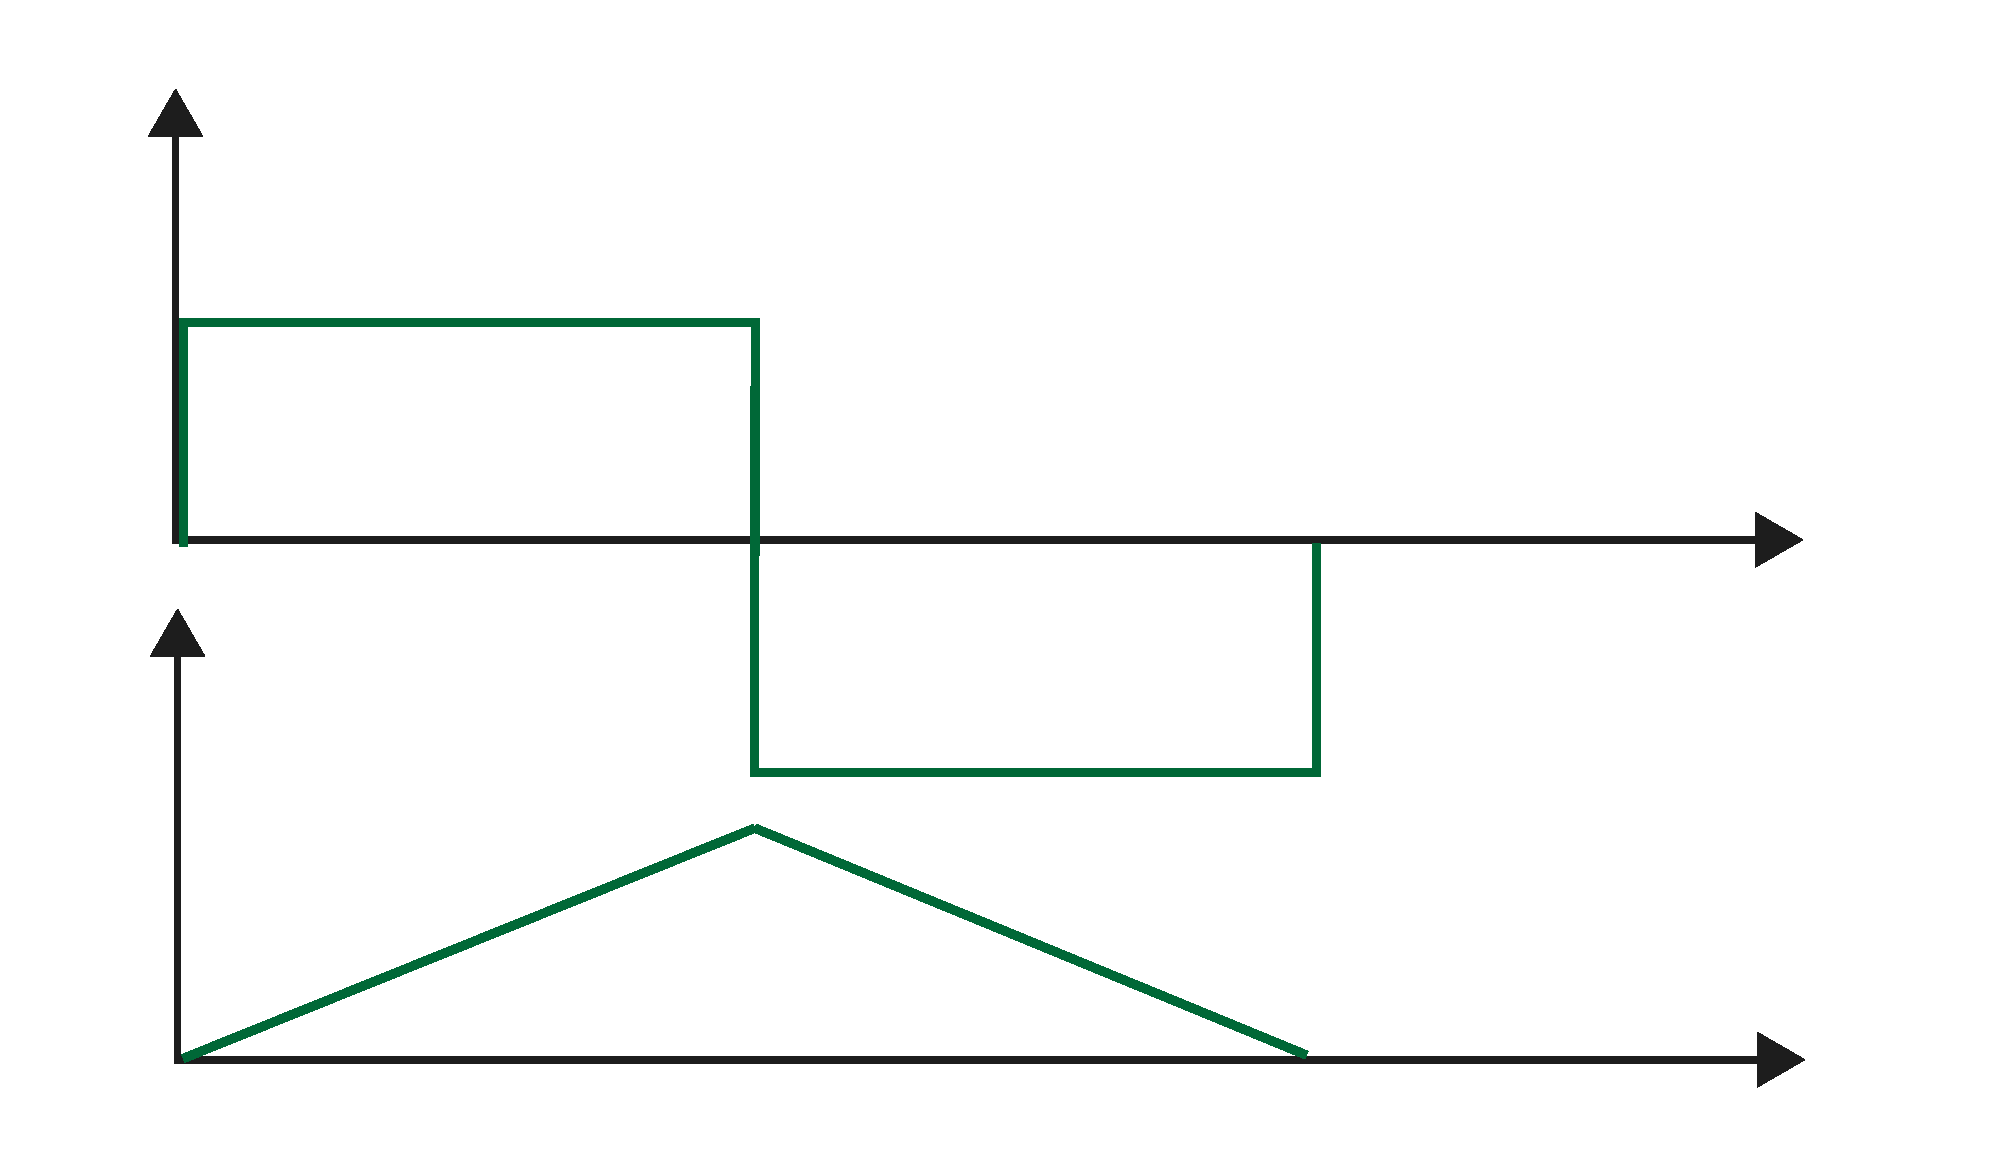
\includegraphics[width=0.4\textwidth]{content/SmoothingFunction.pdf}
	
	\vspace{-2.2cm}
	
	\flushright
	Abgeleiteter Smoothing Kernal
	
	\vspace{.4cm}
	
	Smoothing Kernal	
\end{minipage}

\[ \frac{\mathrm{d}}{\mathrm{d}t}f_s(t) = \int\limits_{-\infty}^{\infty} f(\tau) \cdot \frac{\mathrm{d}}{\mathrm{d}t}\Theta(\frac{\tau - t}{s}) \, \mathrm{d}\tau = -\frac{1}{s} \int\limits_{-\infty}^{\infty} f(\tau) \cdot \Theta'(\frac{\tau - t}{s}) \, \mathrm{d}\tau \]

Wavelet das integriert ein Smoothing Kernal ergibt: Haar-Wavelet ("Abgeleiteter Smoothing Kernal")\\
Daraus Folgt das die DWT oder SWT (besser) für die Approximation der Ableitung der Smoothed Function verwendet werden kann. Wird die SWT verwendet, dann kennt man die Ableitung der Funktion an allen Punkten.
\[ 
	\frac{\mathrm{d}f}{\mathrm{d}t} \approx C(m) \cdot v_{m,n}
	\qquad \qquad
	v_{m,n} =  \int\limits_{-\infty}^{\infty} f(\tau) \psi_{m,n}(\tau) \, \mathrm{d}\tau 
\]
Das Integral vom Smoothing Kernal muss 1 ergeben, damit das Mittel von $f$ gleich bleibt: 
\[ \int \underbrace{\int C(m) \psi_{m,n}(\tau) \,\mathrm{d}\tau}_{\Theta} \,\mathrm{d}t = 1 \]


\subsection{Matlab}
